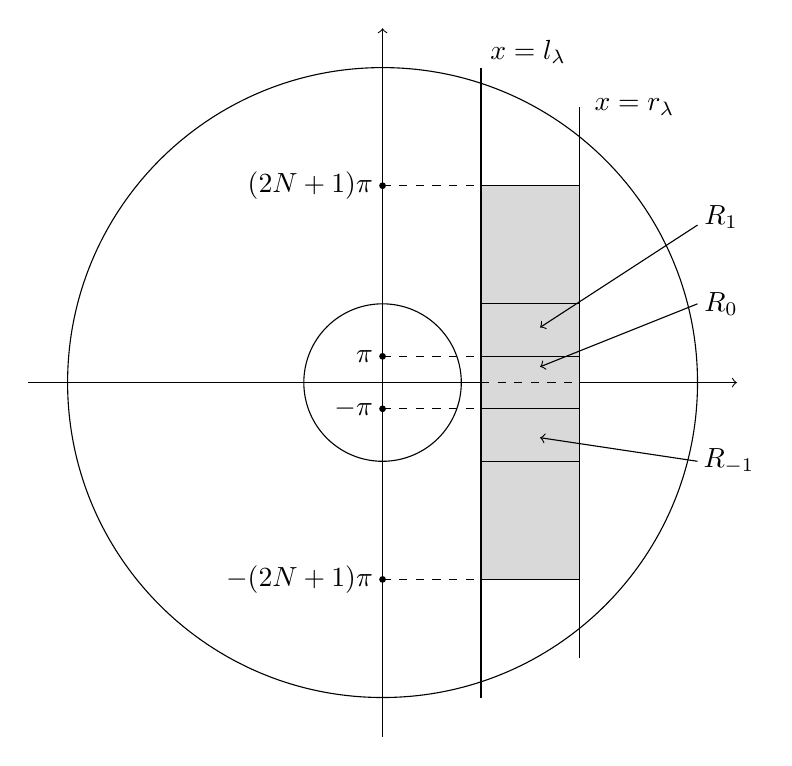
\begin{tikzpicture}
\definecolor{siva}{gray}{0.75}

\draw[->] (-4.5, 0) -- (4.5, 0);
\draw[->] (0, -4.5) -- (0, 4.5);

\draw (0, 0) circle (1);
\draw (0, 0) circle (4);

\fill[gray!30] (1.25, -2.5) rectangle (2.5, 2.5);

\draw (1.25, -4) -- (1.25, 4)
    node[xshift=0.6cm, yshift=0.2cm] {$x = l_\lambda$};
\draw (2.5, -3.5) -- (2.5, 3.5)
    node[xshift=0.7cm] {$x = r_\lambda$};

\draw[dashed] (0, 2.5) -- (1.25, 2.5);
\draw[dashed] (0, 0.333) -- (1.25, 0.333);
\draw[dashed] (0, -0.333) -- (1.25, -0.333);
\draw[dashed] (0, -2.5) -- (1.25, -2.5);

\draw (1.25, 2.5) -- (2.5, 2.5);
\draw (1.25, 1) -- (2.5, 1);
\draw (1.25, 0.333) -- (2.5, 0.333);
\draw[dashed] (1.25, 0) -- (2.5, 0);
\draw (1.25, -0.333) -- (2.5, -0.333);
\draw (1.25, -1) -- (2.5, -1);
\draw (1.25, -2.5) -- (2.5, -2.5);

\filldraw[black] (0, 2.5) circle (1pt)
    node[left]  {$(2N + 1) \pi$};
\filldraw[black] (0, 0.333) circle (1pt)
    node[left]  {$\pi$};
\filldraw[black] (0, -0.333) circle (1pt)
    node[left]  {$-\pi$};
\filldraw[black] (0, -2.5) circle (1pt)
    node[left]  {$-(2N + 1) \pi$};

\draw[->] (4, 2) -- (2, 0.7);
\draw[->] (4, 1) -- (2, 0.2);
\draw[->] (4, -1) -- (2, -0.7);

\node[xshift=0.3cm, yshift=0.1cm] at (4, 2) {$R_1$};
\node[xshift=0.3cm] at (4, 1) {$R_0$};
\node[xshift=0.4cm] at (4, -1) {$R_{-1}$};

\end{tikzpicture}